\documentclass[a4paper]{article}

\usepackage[english]{babel}
\usepackage[utf8]{inputenc}
\usepackage{fullpage}
\usepackage{amsmath}
\usepackage{graphicx}
\usepackage[colorinlistoftodos]{todonotes}
\usepackage{hyperref}
\usepackage{amssymb}
\usepackage{outline} \usepackage{pmgraph} \usepackage[normalem]{ulem}
\usepackage{graphicx} \usepackage{verbatim}
% \usepackage{minted} % need `-shell-escape' argument for local compile

\usepackage[UTF8]{ctex}
\usepackage[inkscapeformat=png]{svg}
\usepackage{enumitem}

\usepackage{listings}

\lstset{
    columns=fullflexible, 
    keepspaces=true, 
    showspaces=false, 
    showtabs=false, 
    breaklines=true, 
    showstringspaces=false, 
    breakatwhitespace=true, 
    basicstyle=\ttfamily\normalsize, 
    framesep=3pt, 
    xleftmargin=6pt, 
    tabsize=4, 
    captionpos=b
    keywordstyle        =   \bfseries,          % 关键字风格
    % commentstyle        =   \rmfamily\itshape,  % 注释的风格, 斜体
    % stringstyle         =   \ttfamily,  % 字符串风格
    flexiblecolumns,                % 别问为什么, 加上这个
    numbers             =   left,   % 行号的位置在左边
    showspaces          =   true,  % 是否显示空格, 显示了有点乱, 所以不现实了
    showstringspaces    =   true, 
    frame               =   lrtb,   % 显示边框
}

\title{
    \vspace*{1.0in}
    \includesvg[width=2.75in]{figures/logo.svg} \\
    \vspace*{1in}
    \textbf{\Huge 面向人工智能研究的计算机技能分享}
    \vspace{0.5in}
}

\author{ \\
    \textbf{\huge userElaina} \\
    \vspace*{1in}
}

\date{\LARGE 2023.12.07}
\setcounter{page}{-1}
\newpage

\begin{document}
\LARGE

\maketitle
\tableofcontents
% \setcounter{page}{0}
\thispagestyle{empty}
\newpage

\section{\LARGE 背景}

MIT: \href{https://missing.csail.mit.edu/}{The Missing Semester of Your CS Education} (\href{https://missing-semester-cn.github.io/}{计算机教育中缺失的一课}).

大学里的计算机课程通常专注于讲授从操作系统到机器学习这些学院派的课程或主题, 而对于如何精通工具这一主题则往往会留给学生自行探索. 学生在受教育阶段就会和这些工具朝夕相处, 在职业生涯中更是如此. 因此, 能够高效地使用这些工具是非常有必要的, 防止浪费时间和精力在本来可以更简单的任务上. 精通这些工具不仅可以更快地使用工具完成任务, 并且可以帮助解决在之前看来似乎非常复杂的问题.

\begin{enumerate}[leftmargin=2cm, itemindent=1cm]
    \item Course overview + the shell
    \item Shell Tools and Scripting
    \item Editors (Vim)
    \item Data Wrangling
    \item Command-line Environment
    \item Version Control (Git)
    \item Debugging and Profiling
    \item Metaprogramming
    \item Security and Cryptography
    \item Potpourri
    \item Q \& A
\end{enumerate}

2023 年\href{https://www.bilibili.com/video/BV1T84y1w7wB}{春夏学期}: 计算机学院朋辈辅学课程;

2023 年\href{https://www.bilibili.com/video/BV1t34y1g7YU}{秋冬学期}: 竺可桢学院学院学业指导中心辅学计划, 程序设计精品课;

ZJU: \href{https://slides.tonycrane.cc/PracticalSkillsTutorial/}{实用技能拾遗}.

\begin{enumerate}[leftmargin=2cm, itemindent=1cm]
    \item 前瞻: 通往 Pro 的第一步
    \item Shell 基础及 CLI 工具推荐
    \item Git / GitHub 及开源基础
    \item Markdown 语法及应用
    \item LaTeX 排版简要介绍
    \item 如何排出规范, 美观的文档
    \item Docker 基础介绍
\end{enumerate}

"很长时间你们都被困在墙内", "miss 的比 ZJU 还要多一点".

包括: 镜像站, 代理, 虚拟环境, Shell, CLI, 后台运行, 发行版, LaTeX 等.

不包括: 如何访问 GitHub 等网站.

\section{\LARGE Environment}

\subsection{\LARGE mirrors}

Tuna, BFSU, HIT, USTC, ..., JLU!

\begin{figure}[hb]
    \centering
    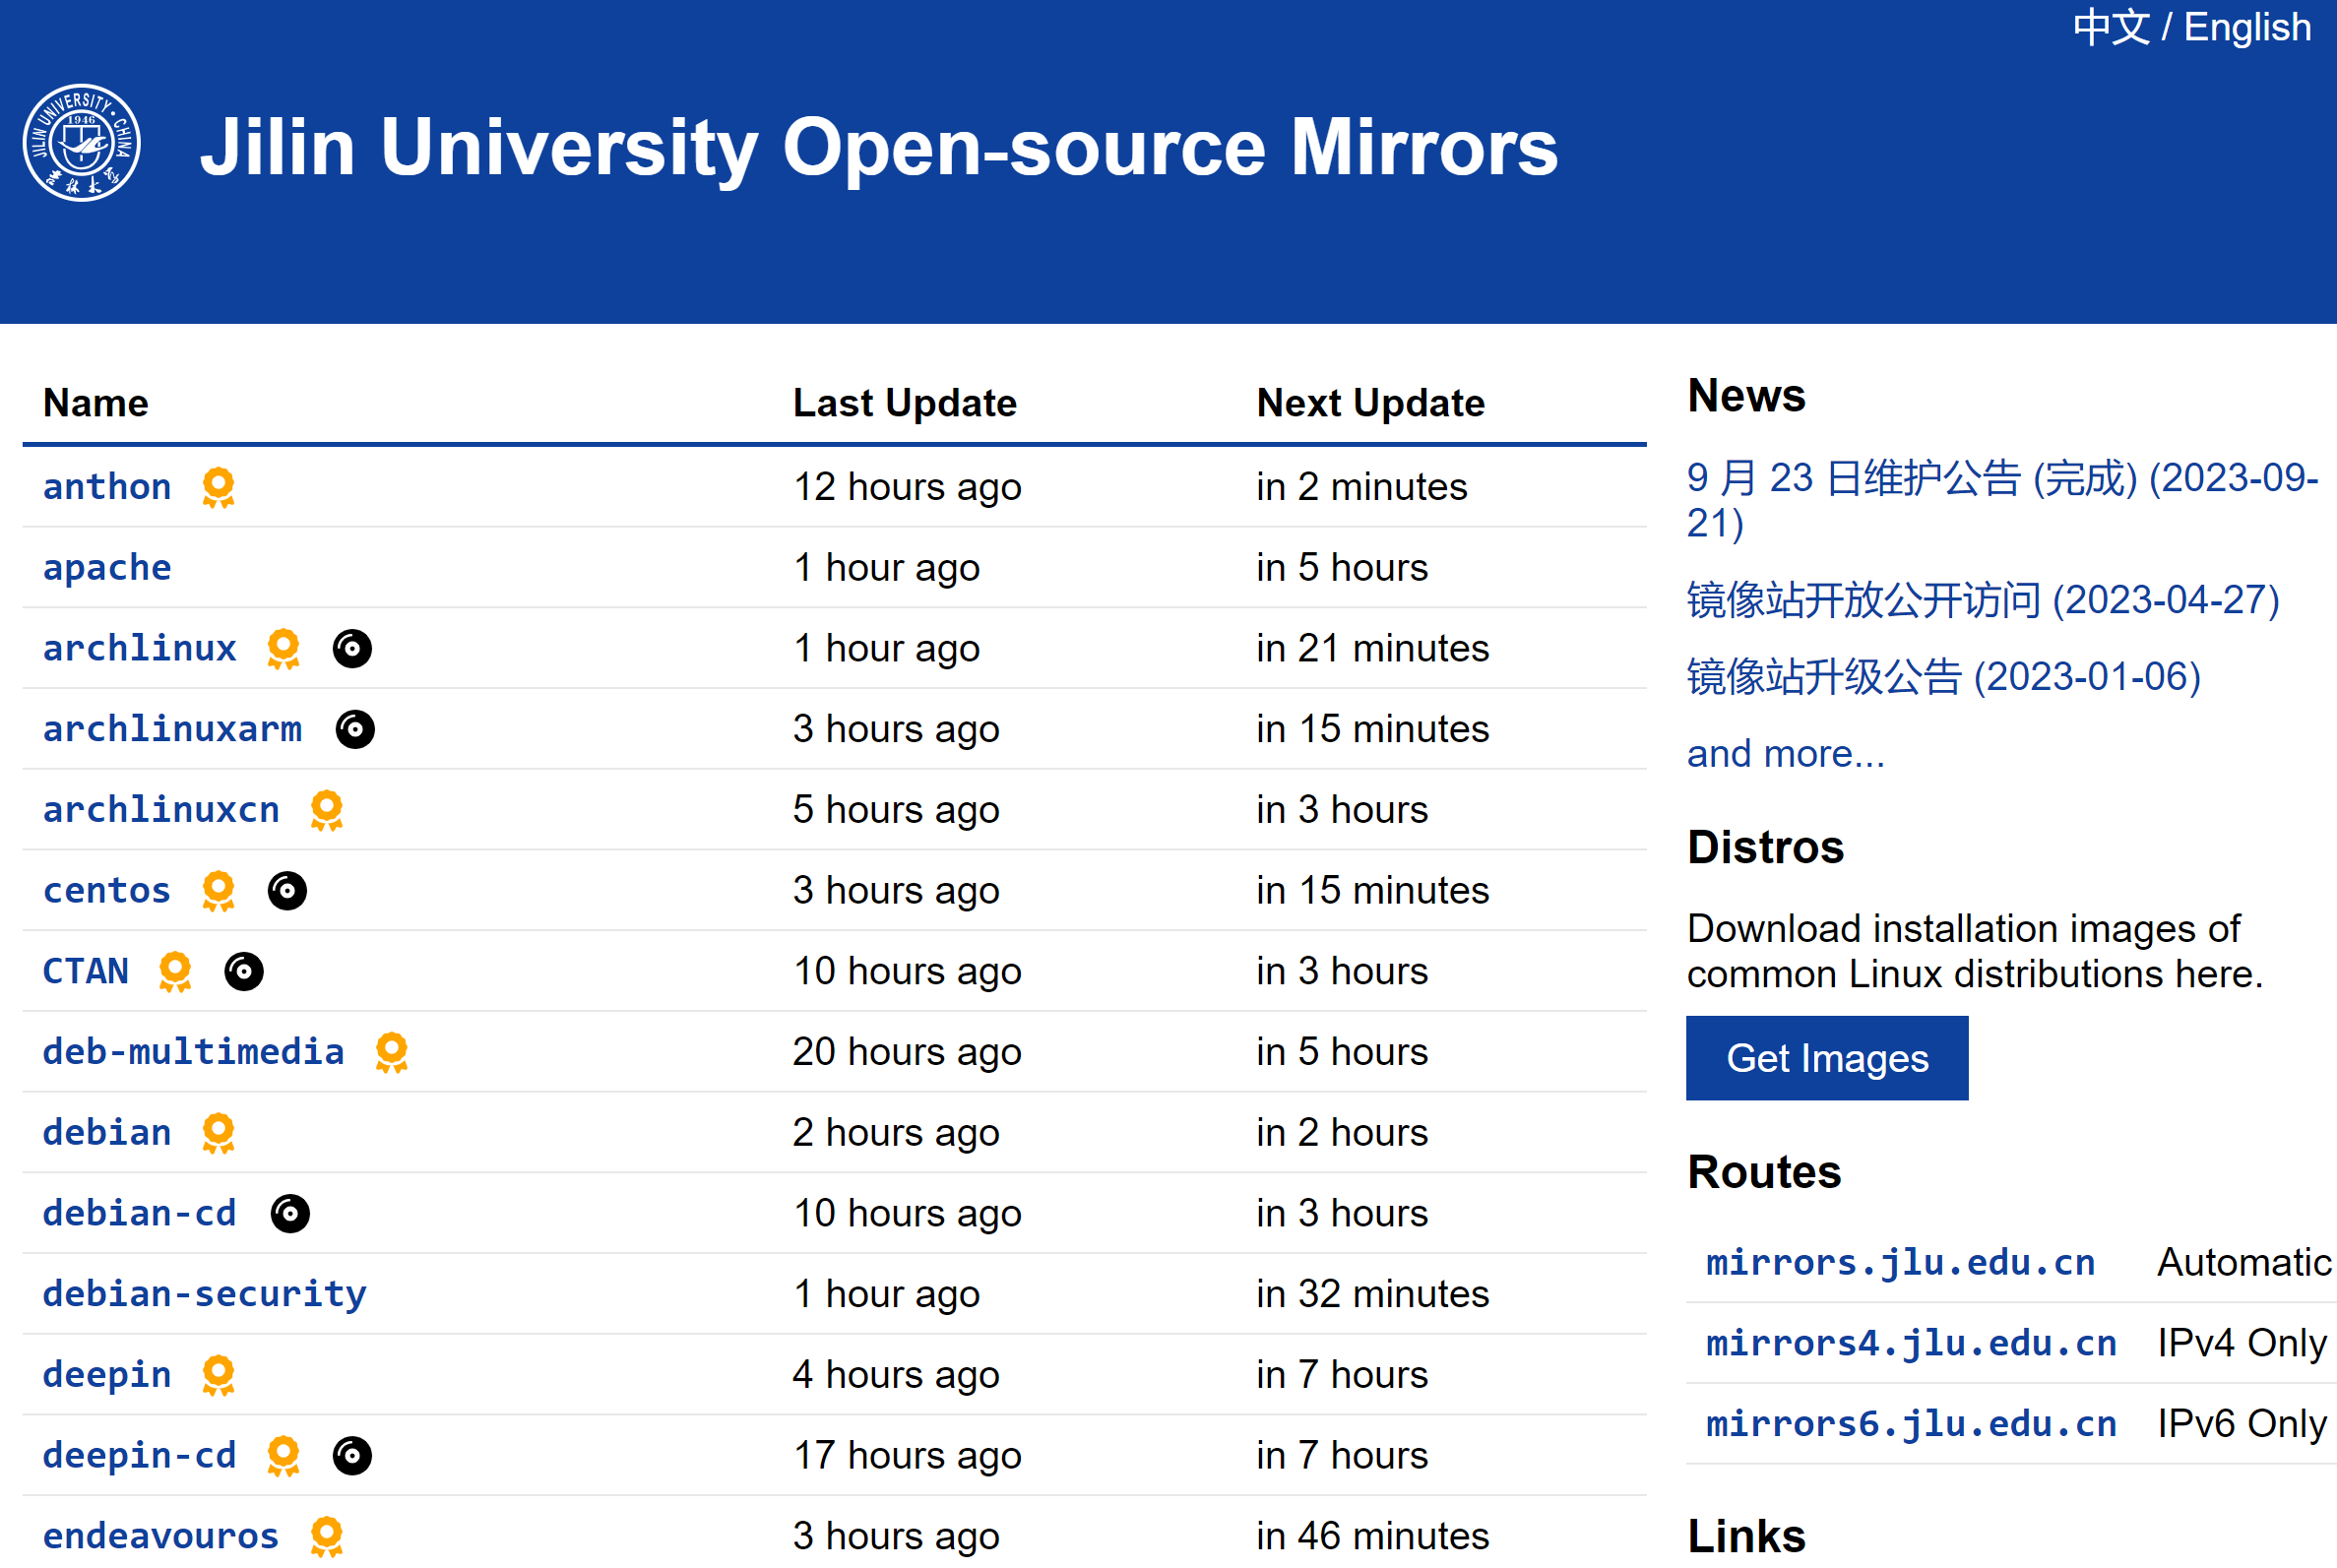
\includegraphics[height=.4\textheight]{figures/mirror.png}
    \caption{https://mirrors.jlu.edu.cn/}
\end{figure}

\begin{enumerate}[leftmargin=2cm, itemindent=1cm]
    \tt
    \item pip install --upgrade numpy \\ -i https://mirrors.jlu.edu.cn/pypi/simple/
    \item ~/.condarc
    \item /etc/apt/source.list
    \item /etc/pacman.d/mirrorlist
    \item pacman-mirrors
\end{enumerate}

\begin{figure}[hb]
    \centering
    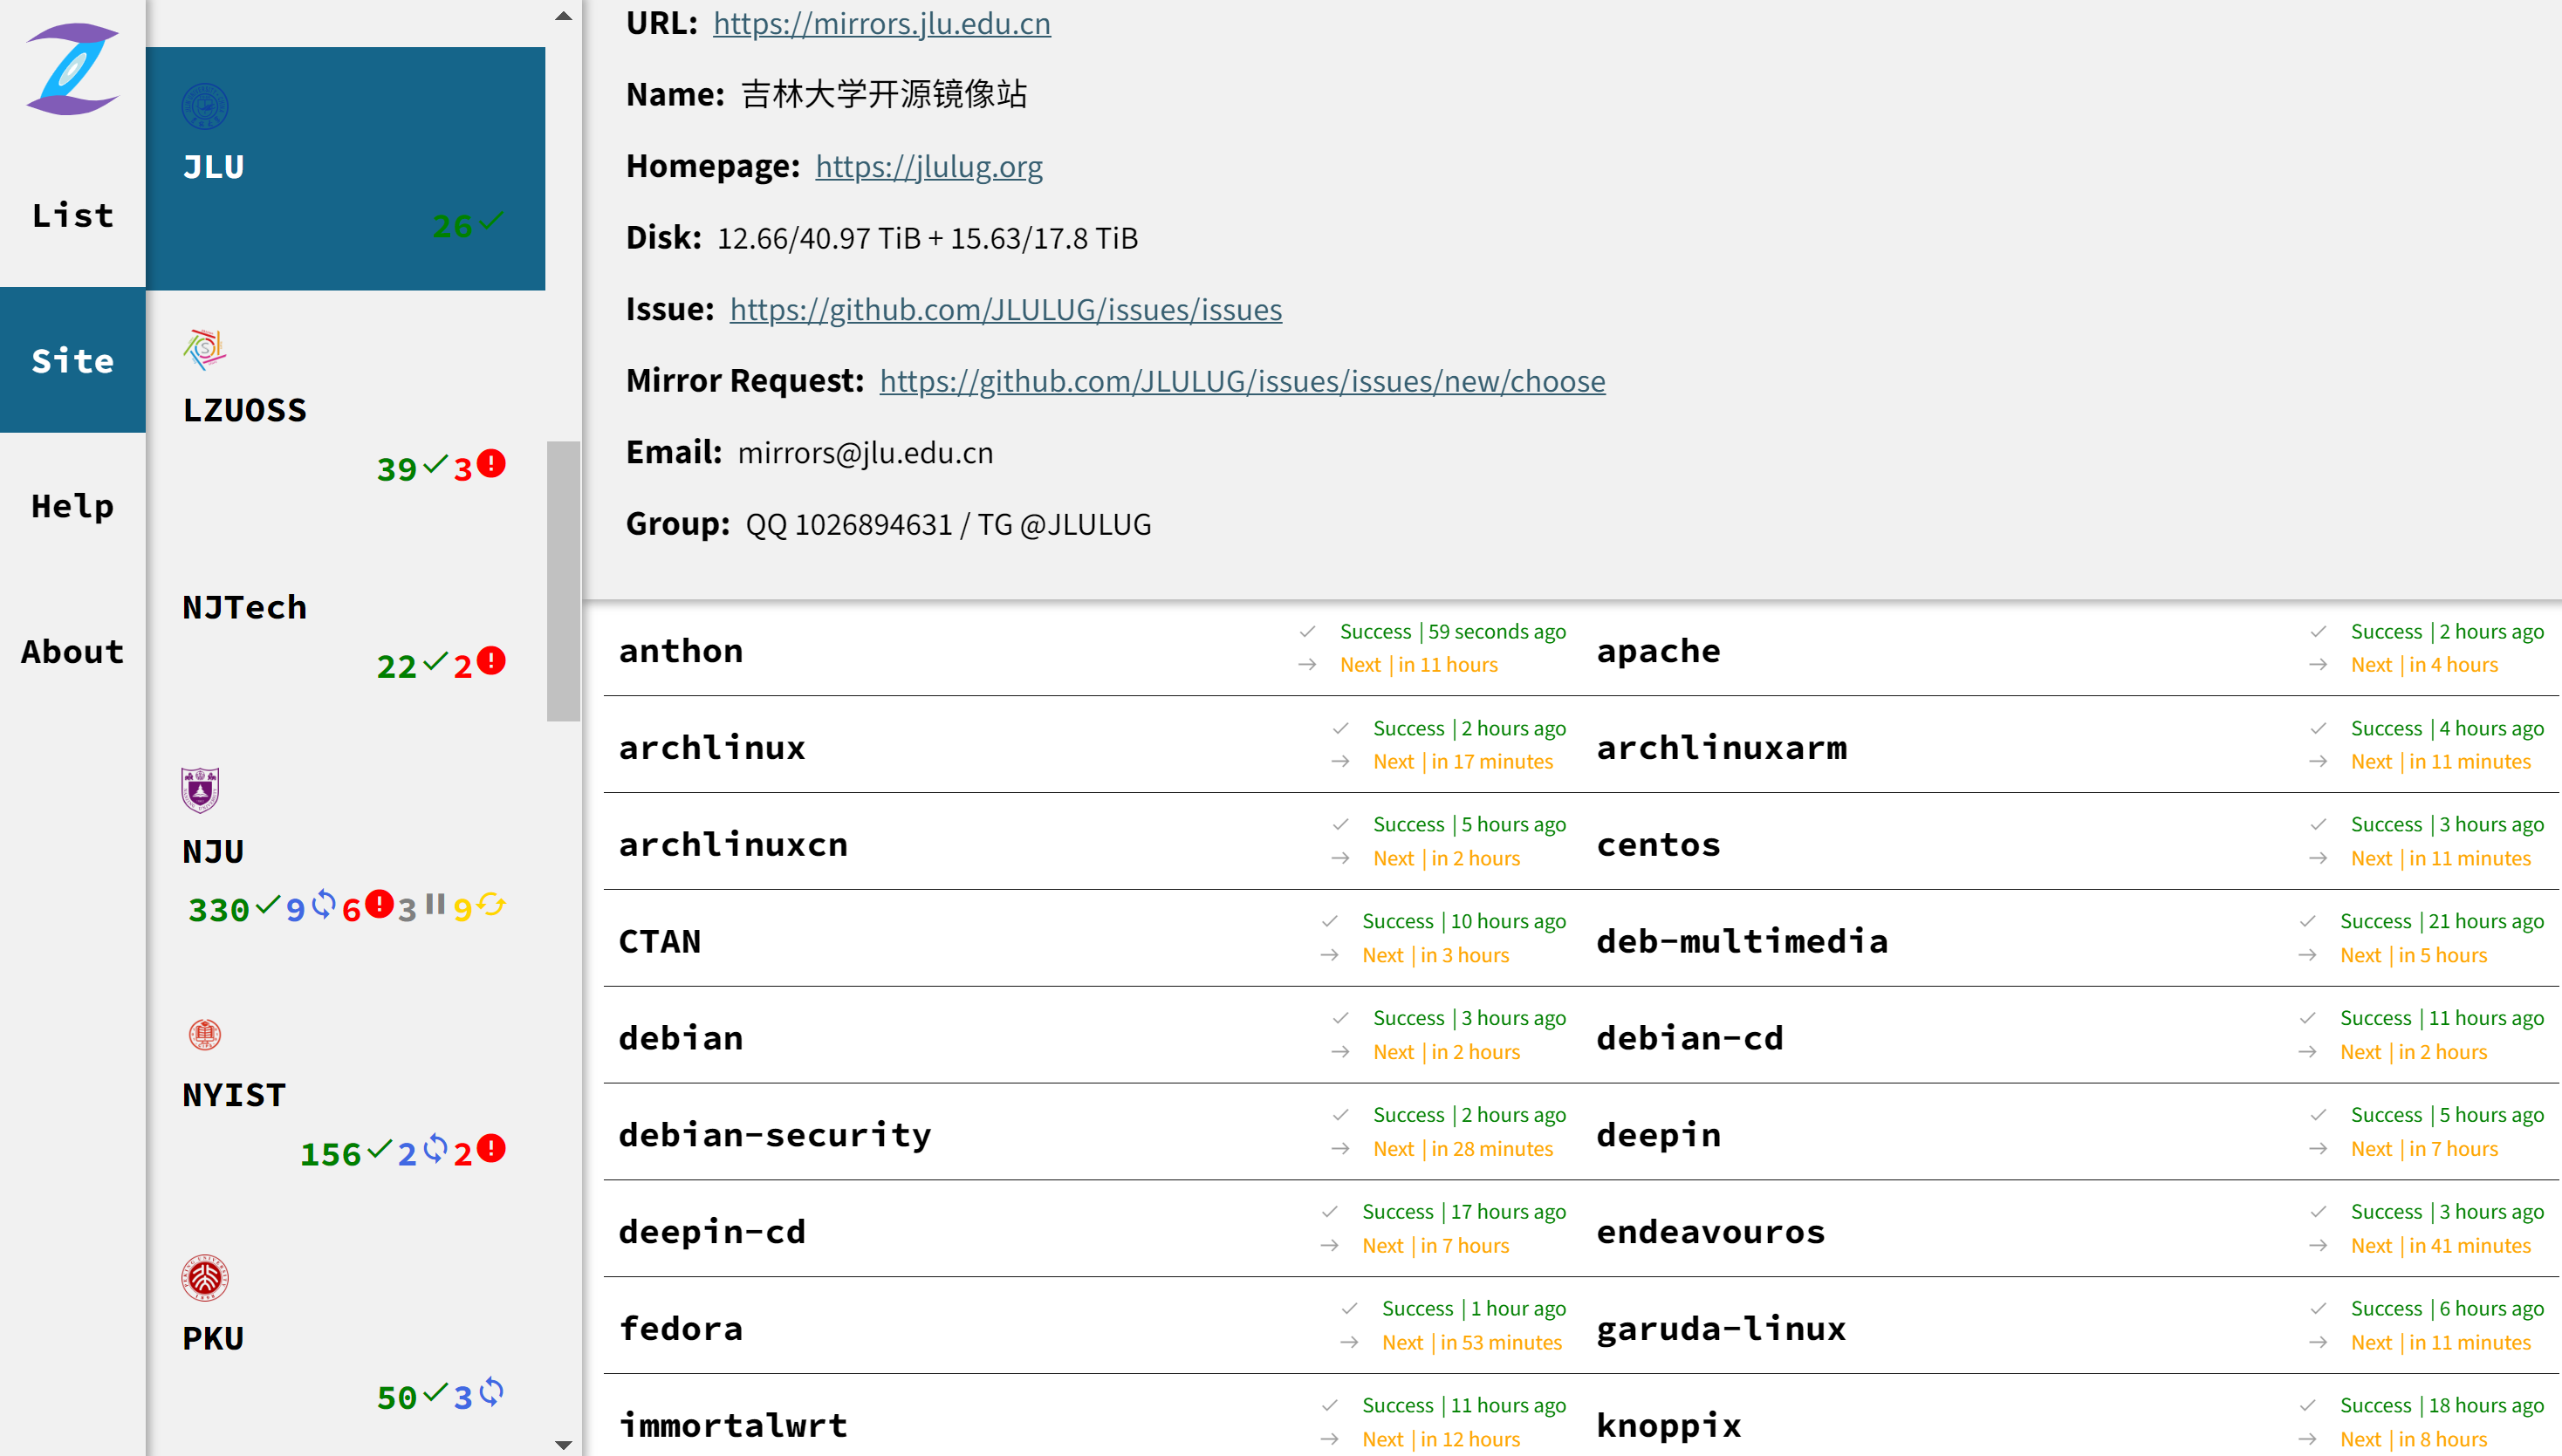
\includegraphics[height=.4\textheight]{figures/mirrorz.png}
    \caption{MirrorZ.org}
\end{figure}

\subsection{\LARGE proxy}

WebVPN 助手: https://greasyfork.org/scripts/395271

包管理器使用代理: https://github.com/rosebe/FUCK-GFW

Transparent Proxy: V2rayA, iptables, OpenWRT, ...

将国际网站伪装成中国网站:

https://github.com/userElaina/this-is-the-China-website

https://greasyfork.org/scripts/461427

\begin{figure}[hb]
    \centering
    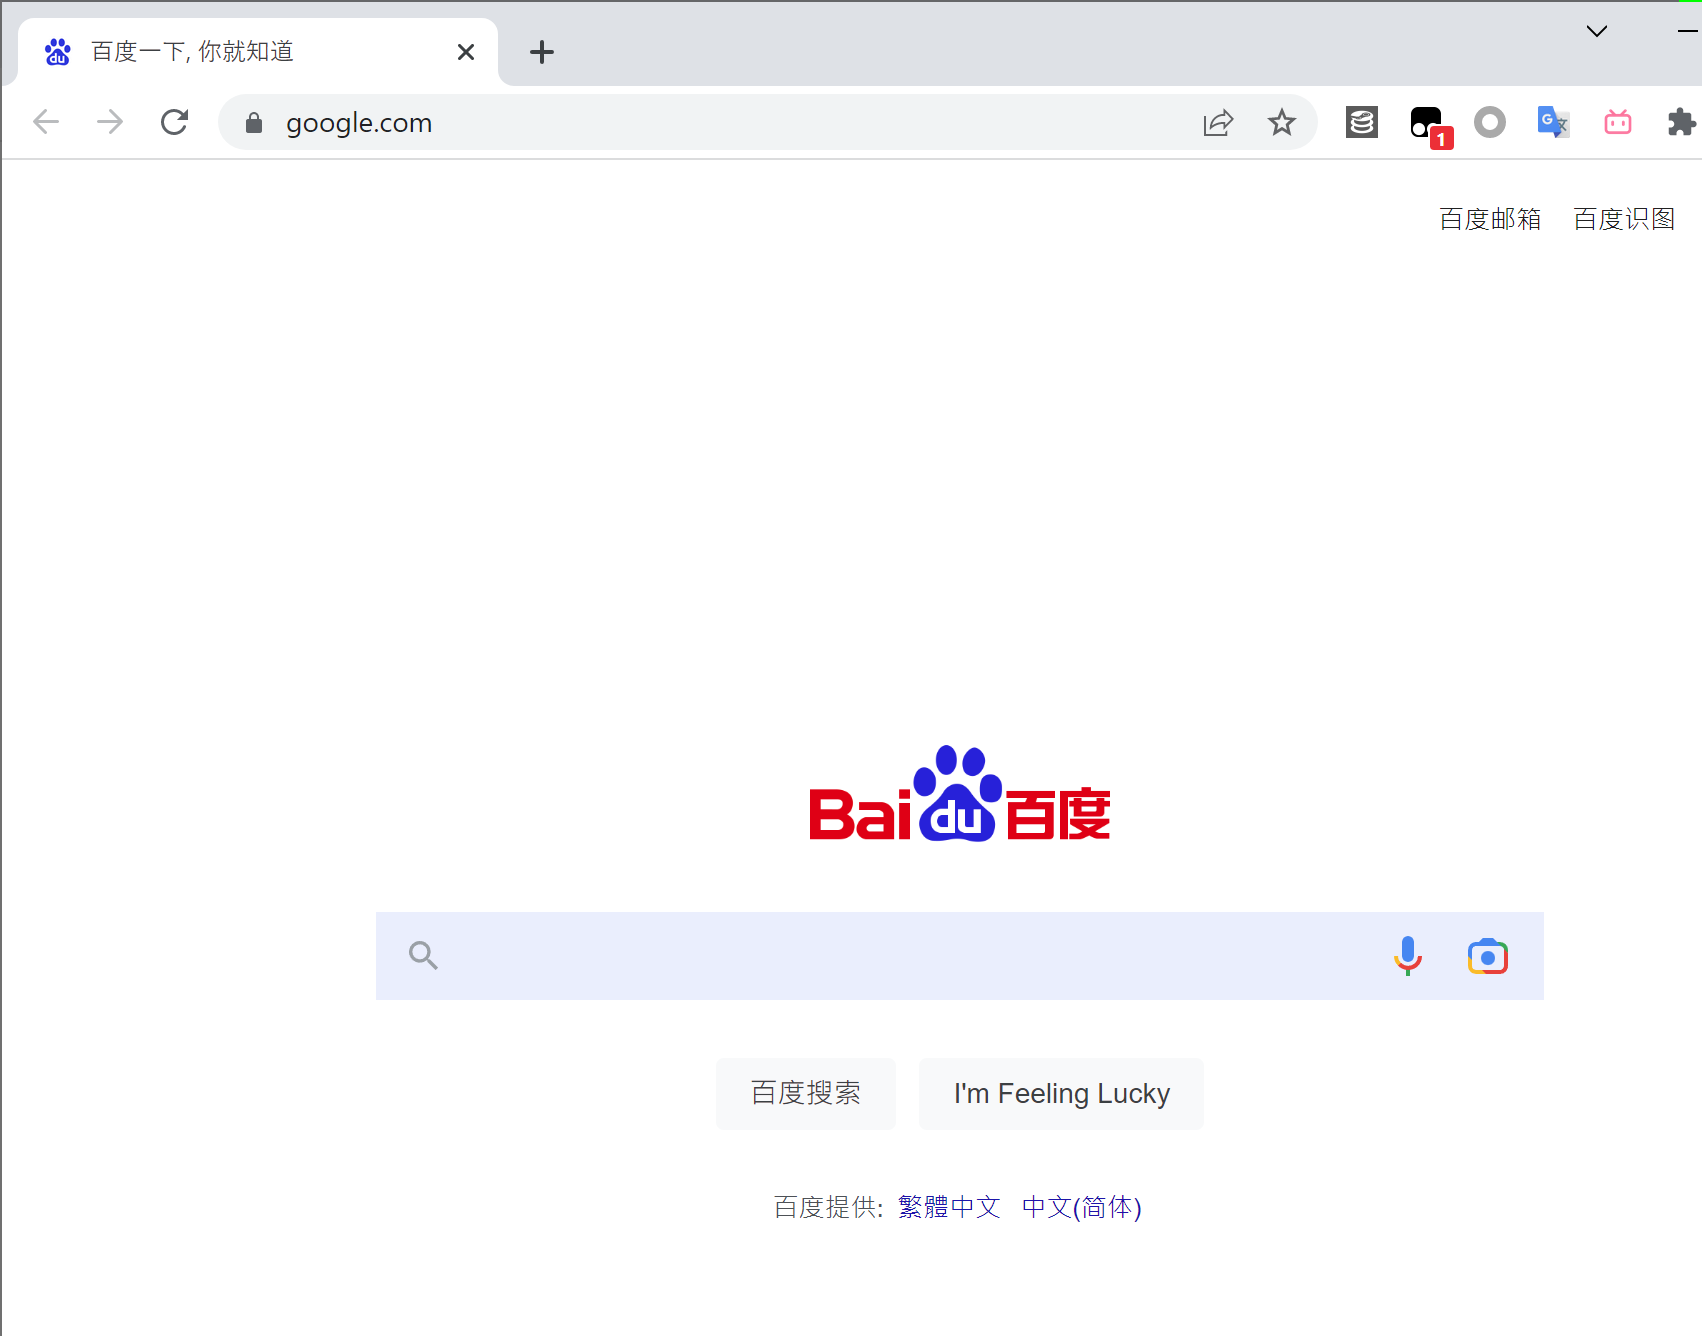
\includegraphics[height=.4\textheight]{figures/google.png}
    \caption{Google}
\end{figure}

\begin{figure}[hb]
    \centering
    
\includegraphics[height=.15\textheight]{figures/search.png}
    \caption{Google search bar}
\end{figure}

\begin{figure}[hb]
    \centering
    
\includegraphics[height=.3\textheight]{figures/ytb.png}
    \caption{YouTube}
\end{figure}

\subsection{\LARGE 虚拟环境}

\subsubsection{\LARGE Python}

{\tt py -m venv ENV\_DIR}

Anaconda / Miniconda

{\tt conda create -n ENV\_NAME python=x.x}

\subsubsection{\LARGE Docker}

其它容器.

\subsubsection{\LARGE Virtual Machine}

WSL, Sandbox, Hyper-V, VirtualBox, VMware, Qemu, PVE, ESXi, ...

Control Panel - Programs - Turn Windows features on or off:

\begin{enumerate}[leftmargin=1cm, itemindent=1cm]
    \item Hyper-V
    \item Windows Hypervisor Platform
    \item Windows Sandbox
    \item Windows Subsystem for Linux
\end{enumerate}

\section{\LARGE Linux}

\subsection{\LARGE Shell}

Shell is not Terminal!

\begin{enumerate}[leftmargin=1cm, itemindent=1cm]
    \item bash: Bourne Again Shell, default.
    \item Zsh: Z Shell, https://ohmyz.sh/.
    \item fish: Friendly Interactive Shell, generates by parsing man pages.
\end{enumerate}

\subsection{\LARGE Help}

\begin{enumerate}[leftmargin=1cm, itemindent=1cm]
    \item {\tt ----help}
    \item man
    \item tldr
    \item RTFM, STFW
\end{enumerate}

\subsection{\LARGE IDE}

编译器: 是将原始语言源代码转换成目标语言计算机程序. gcc, msvc, clang, ...

编辑器: 文本编辑. Vim, NeoVim, VSCode, ...

集成开发环境 (IDE): 能编辑, 构建, 测试, 打包的软件. VS, JetBrains, ...

\subsection{\LARGE CLI}

\begin{enumerate}[leftmargin=1cm, itemindent=1cm]
    \item {\tt ls -ahl}: all, human readable, long listing format
    \item diff, 比较文件
    \item cat, bat, 输出与拼接文件
    \item xxd, hexyl, 十六进制输出文件
    \item find, fd, 查找文件
    \item grep, ripgrep, 搜索文件内容
    \item top, htop, btop, "任务管理器"
    \item make, cmake, 自动化
    \item neofetch, 显示系统信息
    \item FFmpeg, 多媒体处理
\end{enumerate}

\subsection{\LARGE SSH (SCP)}

\begin{enumerate}[leftmargin=1cm, itemindent=1cm]
    \tt
    \item ssh-keygen -t ed25519 -C "userelaina@pm.me"
    \item cat \textasciitilde/.ssh/id\_ed25519.pub
    \item ssh-ed25519 AAAAC3NzaC1lZDI1NTE5AAAAIKmmagvzHfnb NiN3mKrLYqCirEm75But9tKxKas5VX4n userelaina@pm.me
    \item vim \textasciitilde/.ssh/id\_ALGORITHM
    \\ \quad \\
    \item ssh -i \textasciitilde/.ssh/id\_ed25519 -p 50022 user@nas.mil
    \item scp -P 50022 -r ./a/ user@192.168.1.2:\textasciitilde/t1/
\end{enumerate}

\subsection{\LARGE Git (GitHub)}

\begin{enumerate}[leftmargin=1cm, itemindent=1cm]
    \item {\tt git clone https://github.com/opencv/opencv.git}
    \item {\tt git clone git@github.com:opencv/opencv.git}
    \item {\tt git clone --recurse-submodules --remote-submodule https://github.com/bad-apple-lab/Bad-Apple.git}
    \\ \quad \\
    \item GitHub - Settings - SSH and GPG keys
    \item {\tt vim \textasciitilde/.ssh/config}
    \item {\tt ssh -T git@github.com}
\end{enumerate}

\subsection{\LARGE 后台运行}

\begin{enumerate}[leftmargin=1cm, itemindent=1cm]
    \item \sout{\&}
    \item {\tt nohup CMD > LOG 2>\&1 \&}
    \item screen
    \item Tmux
\end{enumerate}

\subsection{\LARGE Distribution}

\begin{enumerate}[leftmargin=1cm, itemindent=1cm]
    \item Debian and Ubuntu
    \item Arch Linux and Manjaro
    \item RHEL and CentOS
    \item Kali Linux and Black Arch Linux
    \item Deepin
\end{enumerate}

\section{\LARGE 硬件}

\subsection{\LARGE 硬件加速}

\subsection{\LARGE 硬件选购}

\section{\LARGE 杂项}

\subsection{\LARGE Markdown}

\subsection{\LARGE LaTeX}

\begin{enumerate}[leftmargin=2cm, itemindent=1cm]
    \item Template
    \item Overleaf
    \item IEEE
\end{enumerate}

\subsection{\LARGE Q \& A}

\begin{center}
    {\Huge Thanks!}
\end{center}

\end{document}
